\chapter*{Abstract}
\thispagestyle{empty}
We evaluate, improve and modernise existing \gls{nlp} methods and adapt specifically for conversations between 2 or more individuals. Specifically, we improve methods for \textbf{\gls{da} classification} and \textbf{topic extraction}.

In \gls{da} classification, the aim is to automatically map sentences in conversations to their appropriate social function, such as ``Hello" $\rightarrow$ greeting. we re-implement, fix, tweak, and modernise an existing classifier by Kumar et al.\cite{kumar2017dialogue} to achieve state of the art performance in the \gls{swda} corpus \cite{swda}, which is commonly used for the evaluation of \gls{da} classifiers.
Our model achieves an accuracy of $\mathbf{84.6 \pm 0.3}$, outperforming the previous state of the art model (83.1\%)\cite{ravi2018self} and even the inter-annotator accuracy between the human annotators who created the \gls{swda} dataset\cite{swda}.

Within the area of topic extraction, the goal is to identify \textit{which} topics are featured within a conversation and \textit{at what times}. We evaluate a large number of existing models and identify their limitations when applied to casual conversations to create a novel topic extraction algorithm.
%, which outperforms the state of the art topic segmentation model BayesSeg. 
Using the standard metric for evaluating topic segmentation, windowDiff, $w_d$, (in which a lower score indicates a better segmentation performance) our algorithm achieves $w_d = \mathbf{0.22 \pm 0.04}$, outperforming previous state of the art BayesSeg\cite{eisenstein2008bayesian} which achieved $w_d = 0.39 \pm 0.06$ when applied to the same conversation transcripts.

Finally, we apply the improved methods to 18,000 conversations from the Spotify podcast dataset\cite{clifton-2020100000} to create and publish a corpus of conversations annotated with linguistic features, enabling future large-scale conversation analysis.

\begin{figure}
    \centering
    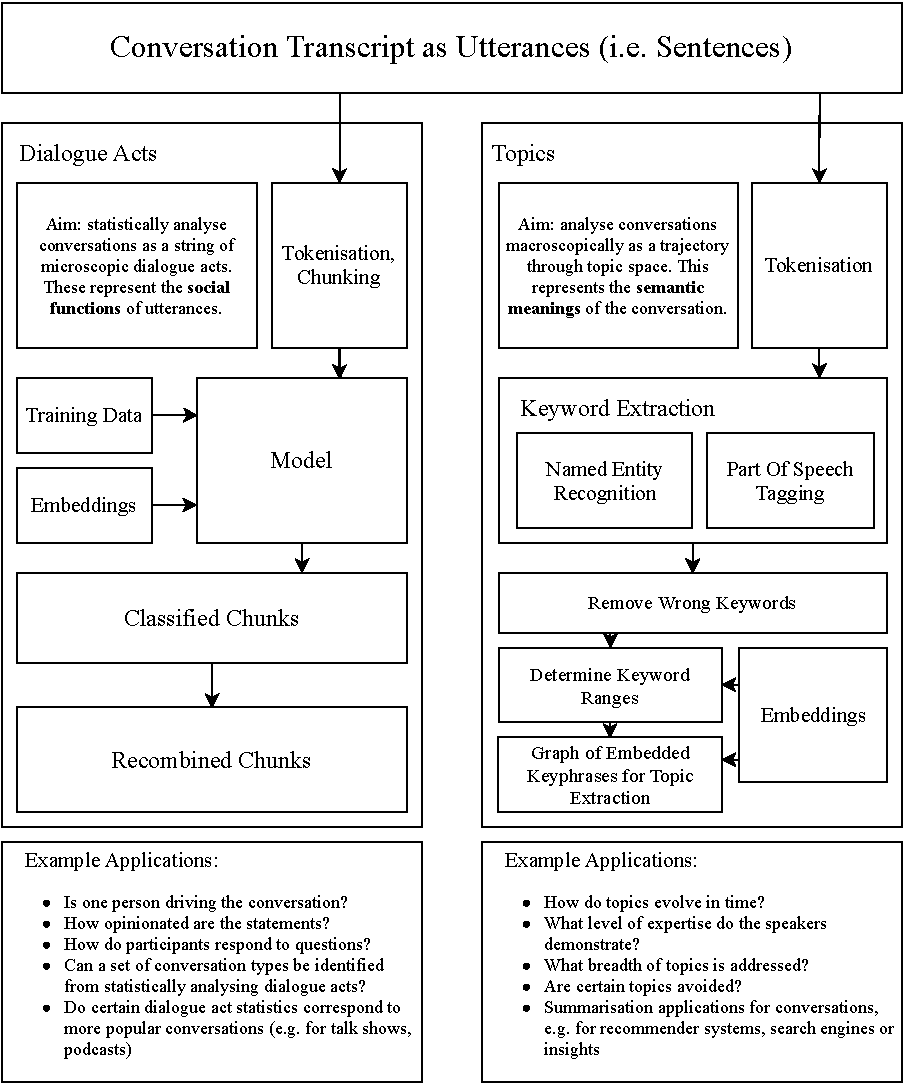
\includegraphics{overview.pdf}
    \caption{Overview of our final methods.}
    \label{fig:overview}
\end{figure}
\glsresetall
\newpage